\subsection{Max Flows and Min Cuts}
Example first:

Given a network of nodes, where each connection has some bandwidth.
\begin{enumerate}
    \item How much data per unit time can be sent from $s$ to $t$?
    \item How much bandwidth must be removed, so that $s$ cannot reach $t$?
\end{enumerate}
The answer for both questions is the same! Max flow = Min cut.

\subsubsection{Flows}
Given a directed graph $G$, with source $s$, target $t$. An $(s,t)-flow$ is a function:
$f:E \rightarrow \mathbb{R}_{\geq 0}$ which satisfies following conservation at all $v \neq s,t$
\[\sum_uf(u \rightarrow v) = \sum_wf(v \rightarrow w)\]
which means flow into $v$ and flow out of $v$.

The ``value'' of the flows, denoted by $|f|$ is
the net flow leaving $s$:
\[|f| = \sum_{w} f(s \rightarrow w) - \sum_{u} f(u \rightarrow s)\]

To simplify notation, define
\[\displaystyle\Delta(f(v)) = \sum_uf(u \rightarrow v) - \sum_wf(v \rightarrow w)\]
as the total net flow out of any vertex $v$.

By conservation:
\[\sum_v\Delta(f(v)) = \Delta(f(s)) + \Delta(f(t)) = 0\]
since any flow leaving vertex must enter some other vertex.

Hence,
\[|f| = \Delta(f(s)) = -\Delta(f(t))\]

Also, given capacity function $c:E \rightarrow \mathbb{R}^{\geq 0}$
that assigns a non-negative capacity $c(e)$ to each edge $e$.
A flow is ``feasible'' (with respect to $c$) if
$f(e) \leq c(e)$, $\forall e \in E$.
A flow $f$ saturates $e$ if $f(e) = c(e)$ and avoid edge $e$ if $f(e) = 0$.
The max flow problem is to \emph{find feasible $f$ s.t. $|f|$ is maximized.}
\begin{figure}[H]
    \centering
    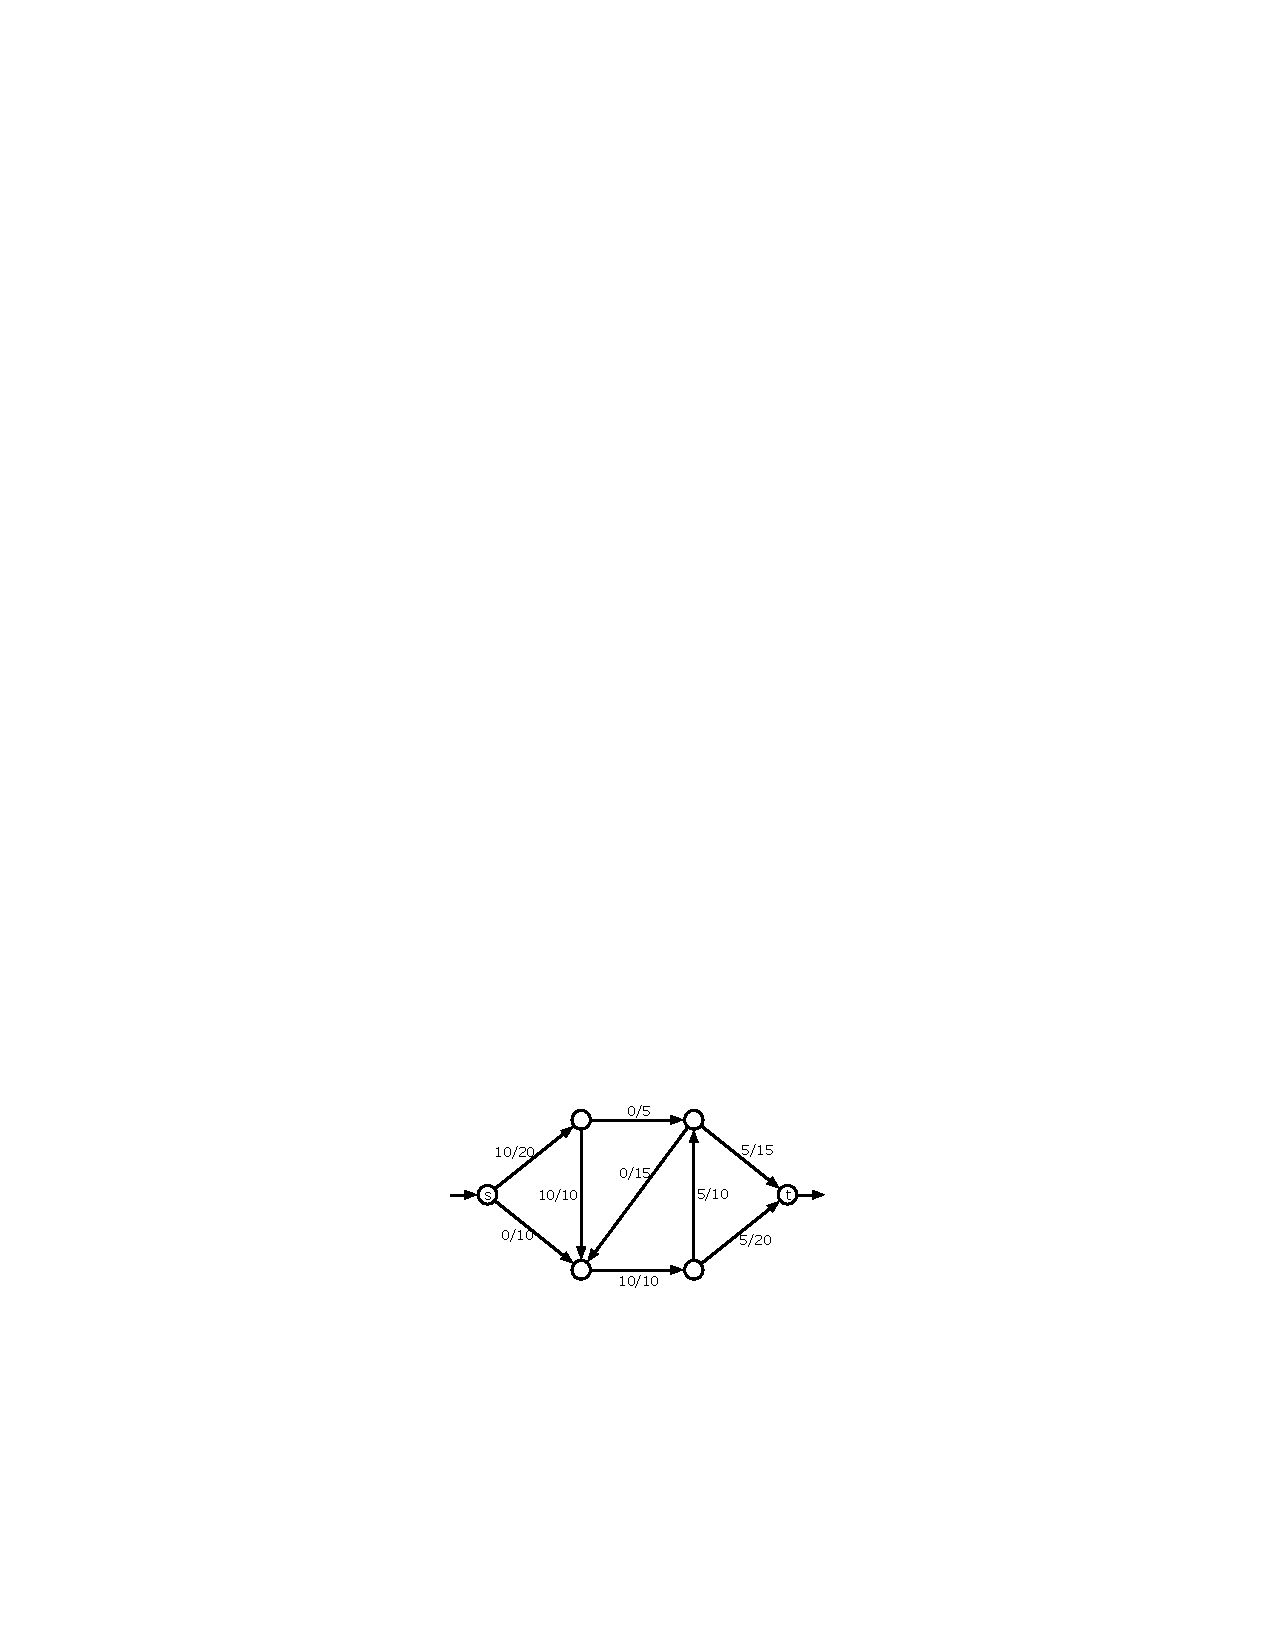
\includegraphics[scale=1.5]{fig/flowExample}
    \caption{An $(s,t)-flow$ with value 10. Each edge is labeled with its flow/capacity.}
    \label{fig:flowExample}
\end{figure}

\subsubsection{Cuts}
An $(s,t)-cut$ is a vertex bi-partition $S,T$,
i.e. $S \cap T = \emptyset$ and $S \cup T = V$, s.t. $s \in S$ and $t \in T$.

The capacity of a cut is the sum of capacities of edges
starting in $S$ and ending in $T$
\[ \|S,T\| = \sum_{v \in S}\sum_{w \in T} c(v \rightarrow w)\]

The min cut problem is to \emph{find cut whos capacity is as small as possible.}
\begin{figure}[H]
    \centering
    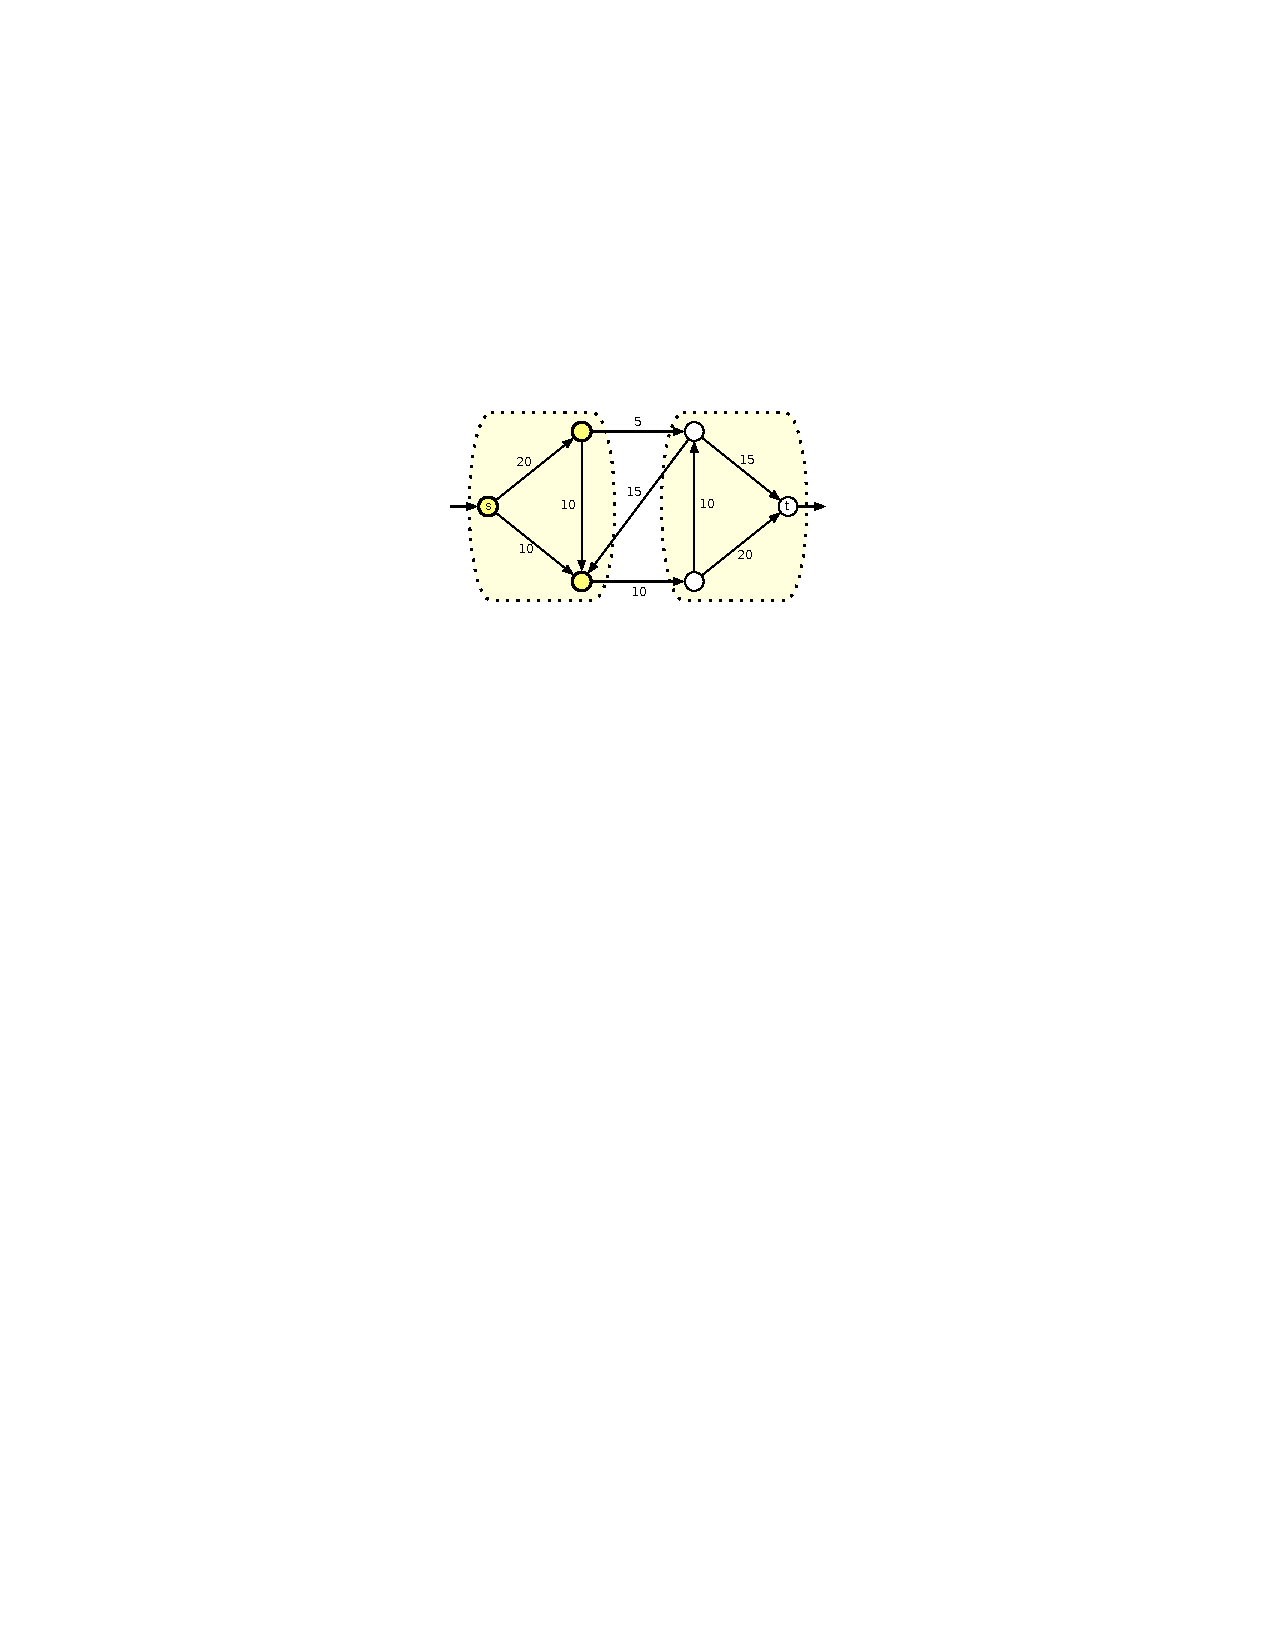
\includegraphics[scale=1.5]{fig/cutExample}
    \caption{An $(s,t)-cut$ with capacity 15. Each edge is labeled with its capacity.}
    \label{fig:cutExample}
\end{figure}

Intuitively, for any feasible $(s,t)-flow$ and any $(s,t)-cut$,
$|f| \leq \|S,T\|$. The proof is as follow:
\begin{align*}
    |f| &= \sum_w f(s \rightarrow w) - \sum_u f(u \rightarrow s) &&\text{by definition}\\
        &= \sum_{v \in S} \left(\sum_w f(v \rightarrow w) - \sum_u f(u \rightarrow v)\right) && \text{by the conservation constraint}\\
        &= \sum_{v \in S} \left(\sum_{w \in T} f(v \rightarrow w) - \sum_{u \in T} f(u \rightarrow v)\right) && \text{removing duplicate edges}\\
        &\leq \sum_{v \in S}\sum_{w \in T} f(v \rightarrow w) && \text{since $f(u \rightarrow v) \geq 0$} \\
        &\leq \sum_{v \in S}\sum_{w \in T} c(v \rightarrow w) && \text{since $f(u \rightarrow v) \leq c(u \rightarrow v)$} \\
        &= \|S,T\| && \text{by definition}
\end{align*}

\observation

$|f| = \|S,T\|$ if and only if:
\begin{itemize}
    \item $f$ avoids every edge from $T$ to $S$;
    \item $f$ saturates every edge from $S$ to $T$.
\end{itemize}

If $|f| = \|S,T\|$, then  $f$ is a max flow and $S,T$ is a min cut.
A max flow saturates all min cuts simultaneously.

\subsubsection{The Maxflow MinCut Theorem}
\begin{theorem}[The Maxflow Mincut Theorem]
    In any flow network with source $s$ and target $t$,
    the value of the maximum $(s,t)-flow$ is equal to
    the capacity of the minimum $(s,t)-cut$.
\end{theorem}

\begin{proof}

To make proof easier, assume capacity function is reduced,
i.e. for $v,w \in V$, either $c(u \rightarrow v) = 0$ or $c(v \rightarrow u) = 0$
(only one of the edges exist). This assumption is easy to enforce,
see \cref{fig:onedirection}.
\begin{figure}[H]
    \centering
    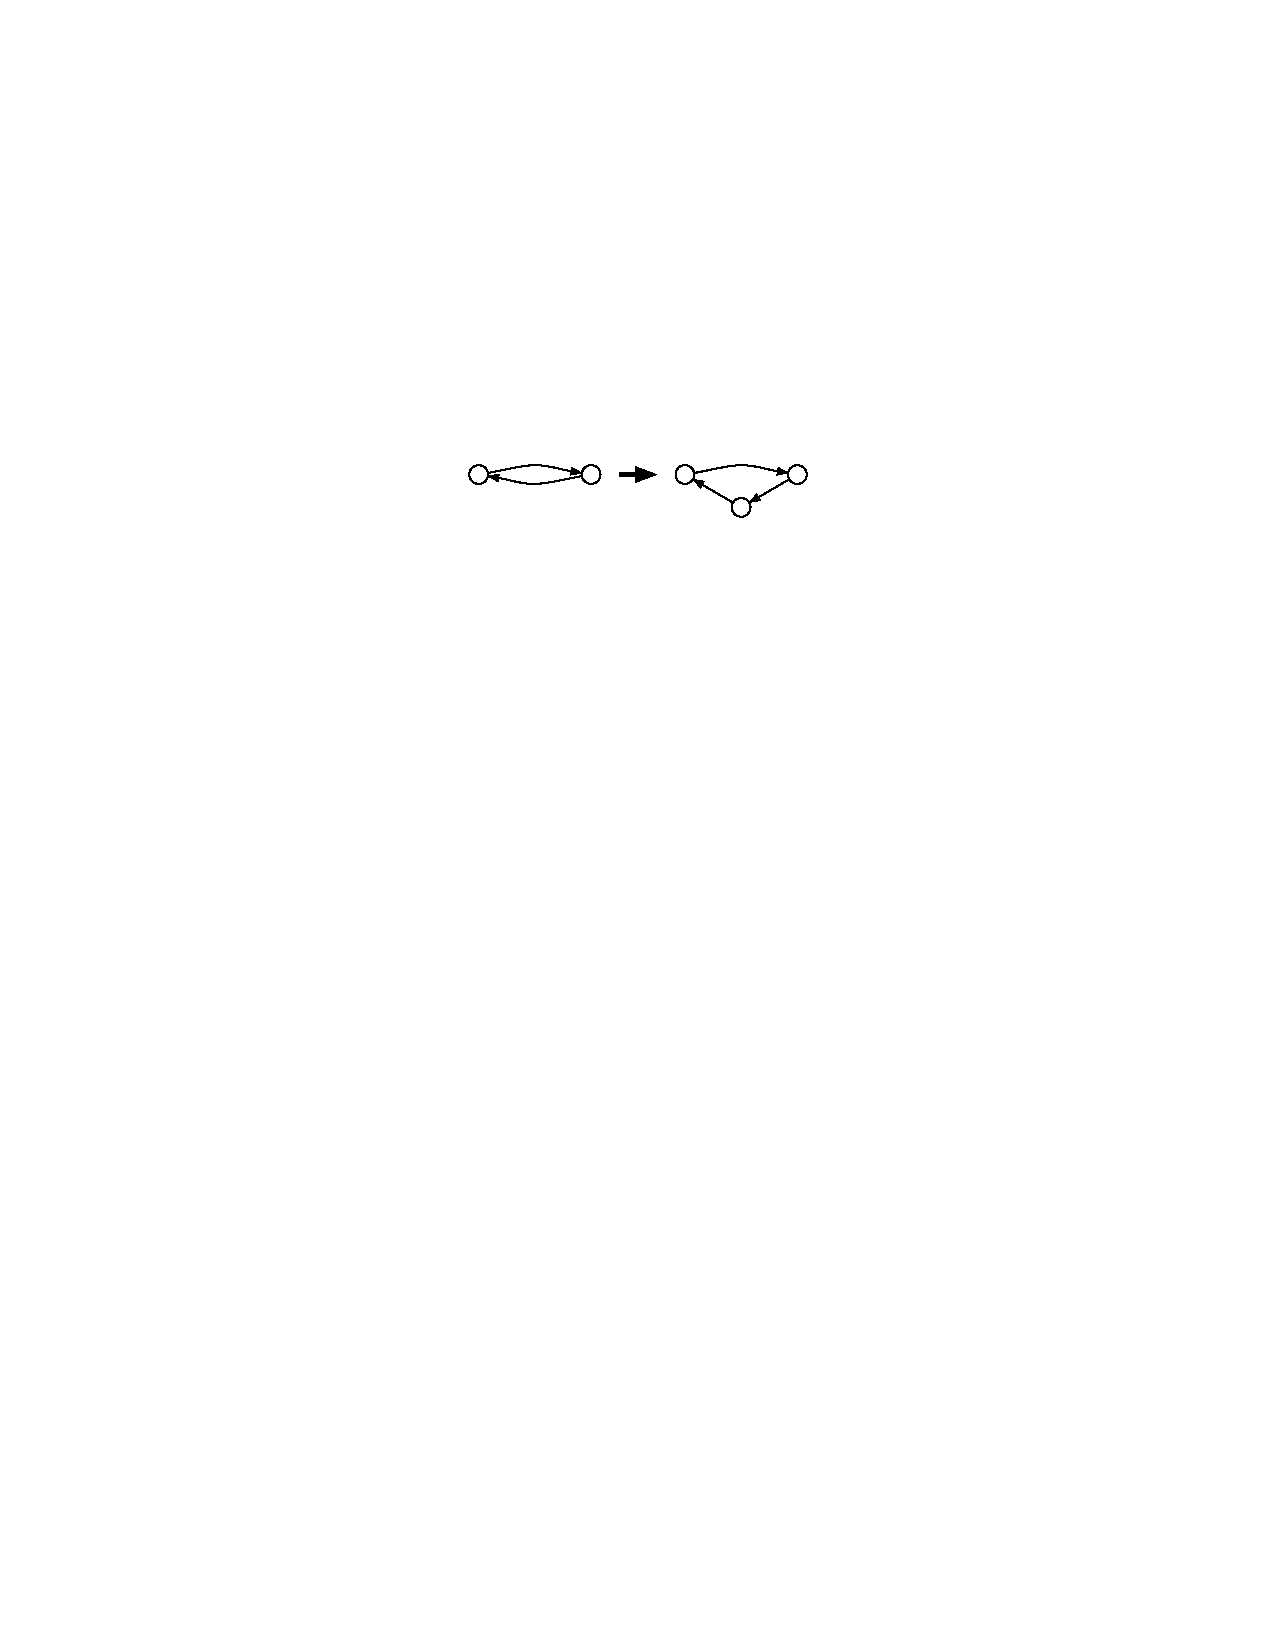
\includegraphics[scale=1.5]{fig/onedirectionassumption}
    \caption{Enforcing the one-direction assumption}
    \label{fig:onedirection}
\end{figure}

Let $f$ be any feasible flow. Define a new capacity function
$c_f:V \times V \rightarrow \mathbb{R}$, called the residual capacity,
as follows:
\begin{equation}
    c_f(u \rightarrow v) = \begin{cases}
        c(u \rightarrow v) - f(u \rightarrow v) & \text{ if } u \rightarrow v \in E\\
        f(v \rightarrow u) & \text{ if } v \rightarrow u \in E\\
        0 & \text{ otherwise } \\
        \end{cases}
\end{equation}
because edge is reduced, an pair can only in one situation.

Since $f \geq 0$ and $f \leq c$, the residual capacities are always non-negative.
Note that, we can have $c_f(u \rightarrow v) > 0$, for $u \rightarrow v \notin E$.
Thus, define residual graph as $G_f = (V, E_f)$,
where $E_f$ is the set of edges with positive residual capacity.
Notice that the residual capacities are not necessarily reduced,
it can have both $c_f(u \rightarrow v) > 0$ and $c_f(v \rightarrow u) > 0$,
as shown in \cref{fig:residualGraphExample}
\begin{figure}[H]
    \centering
    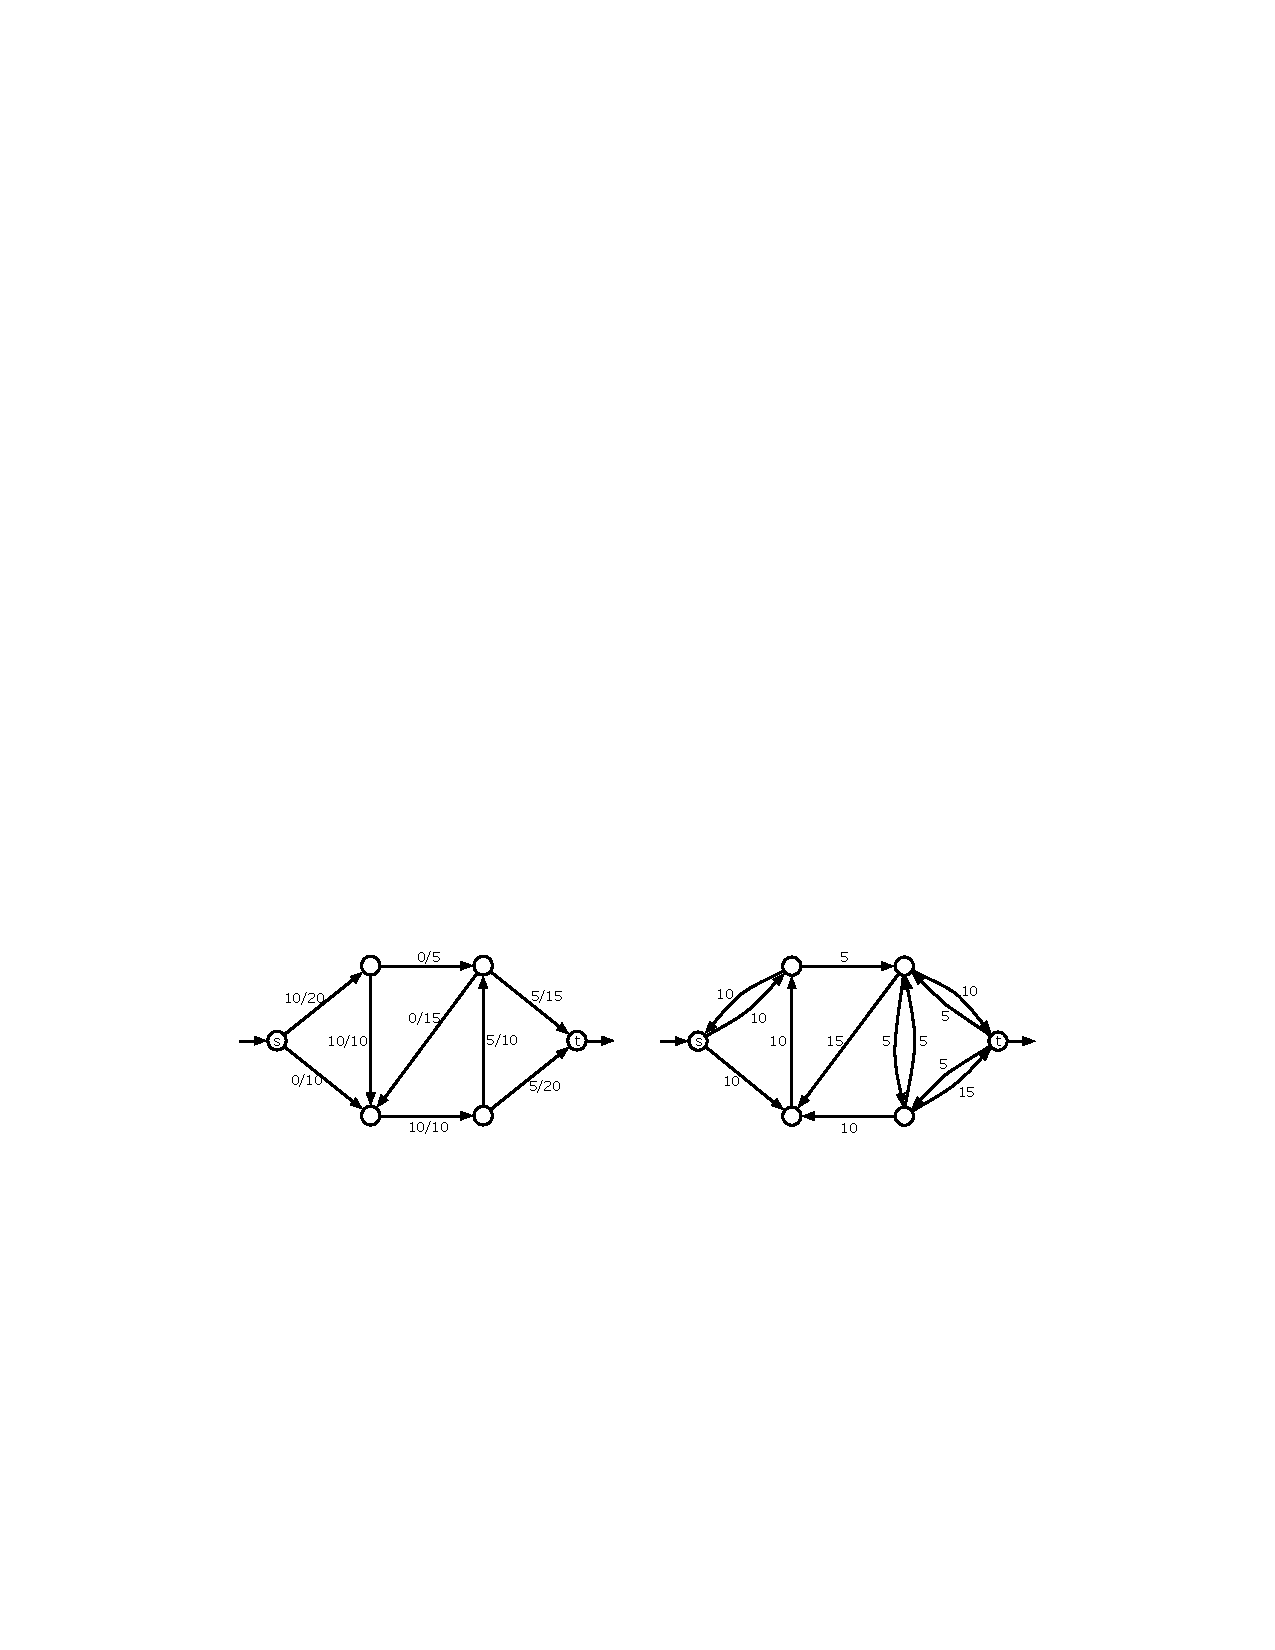
\includegraphics[width=.9\textwidth]{fig/residualGraphExample}
    \caption{A flow $f$ in a weighted graph $G$ and the corresponding residual graph $G_f$.}
    \label{fig:residualGraphExample}
\end{figure}

\begin{enumerate}[label={Case \arabic*}, leftmargin=1in]
    \item There is no path from $s$ to $t$.\\
        Let $S$ be the vertices reachable from $s$ in $G_f$,
        and let $T = V \setminus S$. \\
        Then $(S,T)$ is clearly a cut.\\
        For any $u \in S$ and $v \in T$, we have 
        \[c_f(u \rightarrow v) = (c(u \rightarrow v) - f(u \rightarrow v)) + f(v \rightarrow u) =  0 \text{ , }\]
        \begin{itemize}
            \item If $u \rightarrow v \in E$, then $c(u \rightarrow v) = 0$, i.e. saturated.
            \item if $v \rightarrow u \in E$, then $f(v \rightarrow u) = 0$, i,e, avoided.
        \end{itemize}
        So $f$ avoids every edge from $T$ to $S$ and saturates all edges from $S$ to $T$.\\
        Hence, $|f| = \|S,T\| \Rightarrow f \text{ is max flow, } S,T \text{ is min cut. }$
    \item There is a path $s = v_0 \rightarrow v_1 \rightarrow \cdots \rightarrow v_r = t$ in $G_f$.\\
        Refer to such path as an augmenting path.
        Let $F = \min_i c_f(v_i \rightarrow v_{i+1})$ denote the maximum
        amount can pass through this augmenting path.
        Define a new flow function $f^\prime:E \rightarrow \mathbb{R}$ as follows:
        \begin{equation}
            f^\prime(u \rightarrow v) =
            \begin{cases}
                f(u \rightarrow v) + F & \text{ if } u \rightarrow v \text{ is in the augmenting path } \\
                f(u \rightarrow v) - F & \text{ if } v \rightarrow u \text{ is in the augmenting path } \\
                f(u \rightarrow v) & \text{ otherwise }
            \end{cases}
        \end{equation}
        To prove that the flow $f^\prime$ is feasible with respect to original capacities $c$,
        we need to verify that $f^\prime \geq 0$ and $f^\prime \leq c$ for all edges.

        Consider and edge $u \rightarrow v \in G$.
        \begin{itemize}
            \item If $u \rightarrow v$ is in augmenting path,
                then $f^\prime(u \rightarrow v) > f(u \rightarrow v) \geq 0$ and
                \begin{align*}
                    f^\prime(u \rightarrow v) &= f(u \rightarrow v) + F && \text{ by definition of $f^\prime$ } \\
                                              &\leq f(u \rightarrow v) + c_f(u \rightarrow v) && \text{ by definition of $F$ } \\
                                              &= f(u \rightarrow v) + c(u \rightarrow v) - f(u \rightarrow v) && \text{ by definition of $c_f$ } \\
                                              &= c(u \rightarrow v)
                \end{align*}
            \item If $v \rightarrow u$ is in the augmenting path,
                then $f^\prime(u \rightarrow v) < f(u \rightarrow v) \leq c(u \rightarrow v)$,
                which implies that
                \begin{align*}
                    f^\prime(u \rightarrow v) &= f(u \rightarrow v) - F && \text{ by definition of $f^\prime$ } \\
                                              &\geq f(u \rightarrow v) - c_f(u \rightarrow v) && \text{ by definition of $F$ } \\
                                              &= f(u \rightarrow v) - f(u \rightarrow v) && \text{ by definition of $c_f$ } \\
                                              &= 0
                \end{align*}
            \item If $u \rightarrow v$ nor $v \rightarrow u$ is in augmenting path, nothing change.
        \end{itemize}
\end{enumerate}
Finally, we observe that only the first edge in augmenting path leaves $s$,
so $|f^\prime| = |f| + F > |f|$. Hence, $f$ is not a max flow.

We proved:
\emph{For feasible $f$, let $S$ be reachable set from $s$ in $G_f$, $f$ is max flow,
if and only if $t \notin S$.
If $t \notin S$, $|f| = \|S, V \setminus S\|$ and so $\|S, V \setminus S\|$ is min cut.}
\end{proof}

\subsubsection{Ford-Fulkerson Algorithm}
Maxflow Mincut theorem proof gives an algorithm to compute max flow and hence min cut.
\begin{enumerate}
    \item Initially set $G_f = G$;
    \item Find any $s,t$ path $P$ in $G_f$;
    \item Augment $f$ along $P$, update $G_f$ and repeat until no $s,t$ path.
\end{enumerate}
The question is: how long does this algorithm takes?

\begin{theorem}[Integrality Theorem]
    If all capacities in a flow network are integers, then there is a maximum
    flow such that the flow through every edge is an integer.
\end{theorem}

\analysis Let $f^*$ be max flow.
Each time Ford-Fulkerson's augments, flow increases by at least 1.
Thus, augmenting takes \bigO{|E|} time.
Total time: \bigO{|E||f^*|} time.

However, Ford-Fulkerson might alternate between pushing 1 unit of flow
along the augmenting path back and forth, as shown in \cref{fig:ffexample}.
\begin{figure}[H]
    \centering
    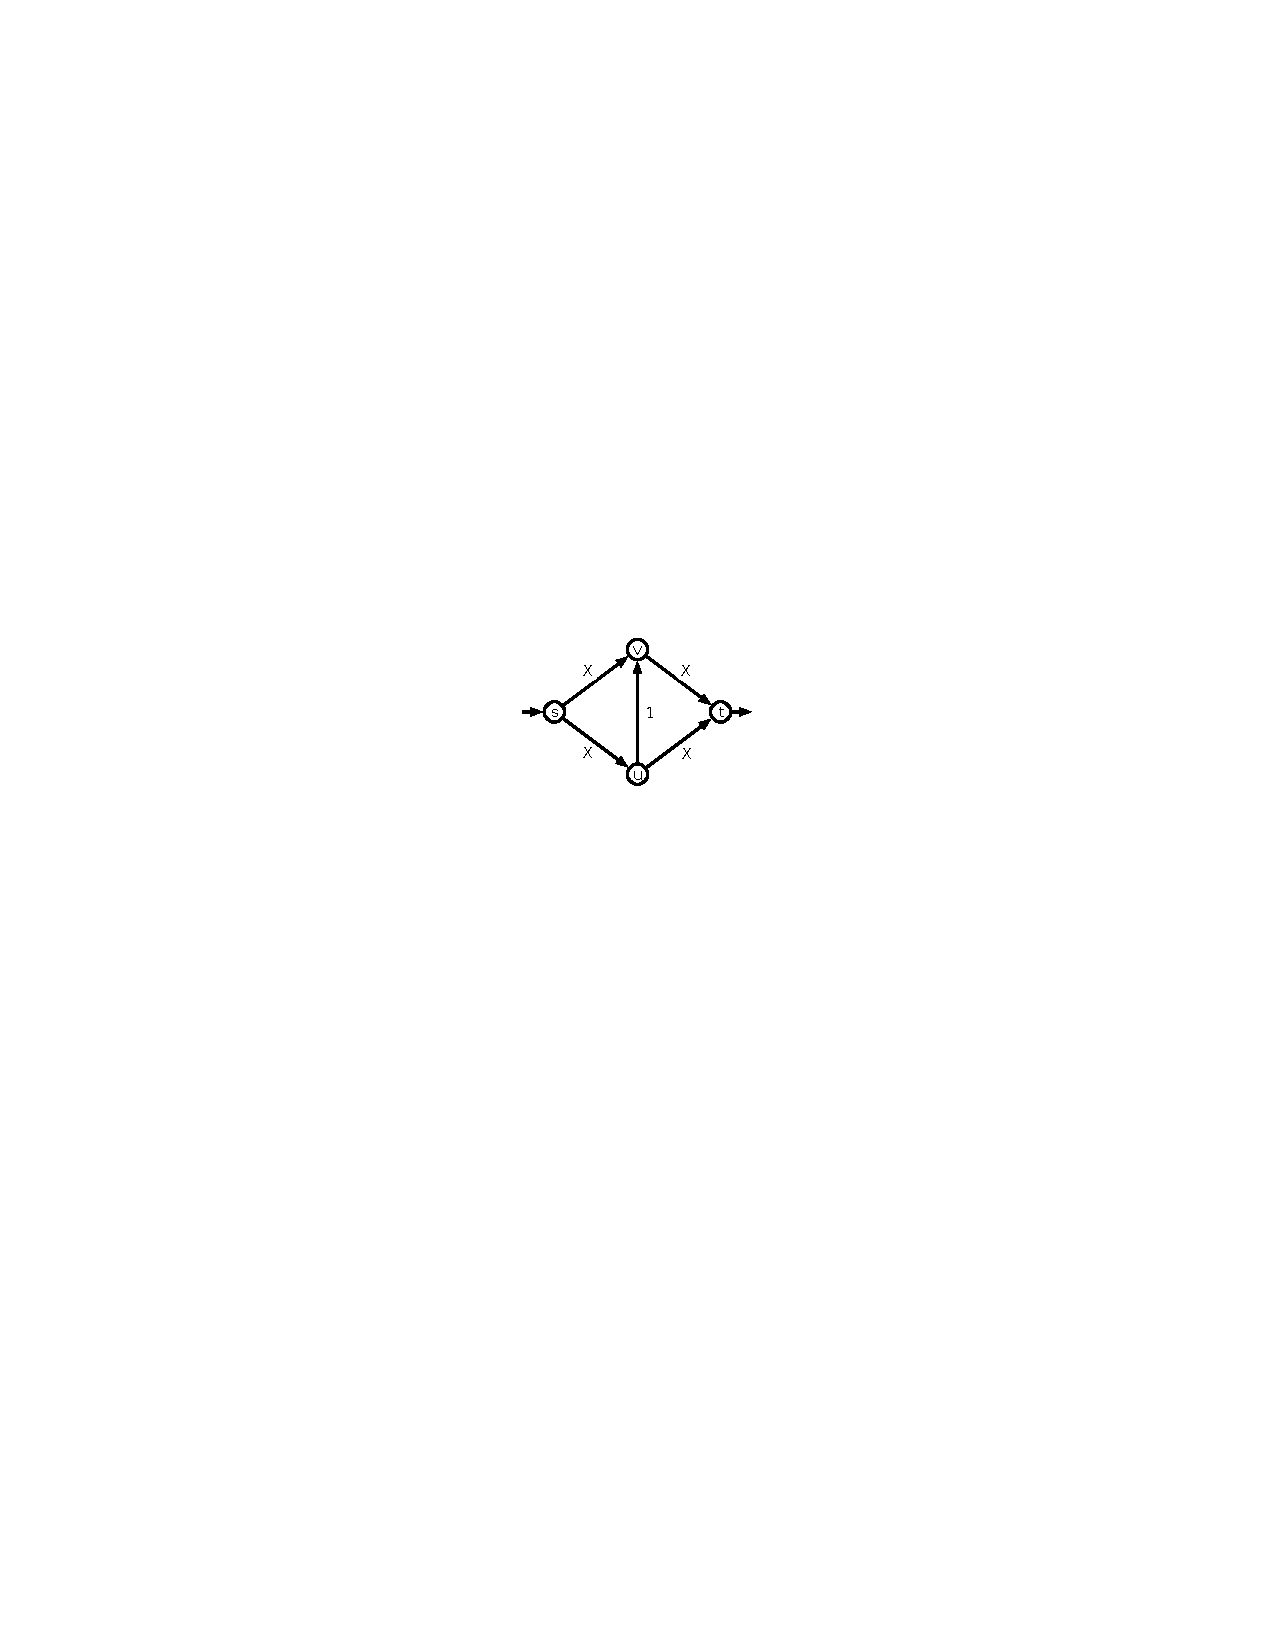
\includegraphics[scale=1.2]{fig/ffexample}
    \caption{A bad example for the Ford-Fulkerson algorithm}
    \label{fig:ffexample}
\end{figure}

To avoid this situation, we can choose (Edmands-Karp algorithm)
\begin{itemize}
    \item path with largest bottleneck;
    \item path with shortest number of edges.
\end{itemize}
For more information, see Chapter 23.6 in Jeff's notes.

In conclusion, Ford-Fulkerson's algorithm takes \bigO{X} time where
the maximum flow value $|f^*| = 2X$, but the input size is \bigO{\log X},
thus, Ford-Fulkerson is actually exponential in the input size.

\subsubsection{Application of Max Flow}
\begin{itemize}
    \item Edge disjoint path (edp).\\
        Given directed grpah $G$, want max number of edge disjoint
        $s-t$ paths (note that it may share vertices).
        Let $K$ be the max number.\\
        Solution: Assign capacity 1 to all edges, compute max flow $f^*$,
        then $|f^*| = k$.
    \item Vertex capacities.\\
        Also given vertex capacities, $c(v)$ for each $v \in V$,
        want max flow with additional requirement that total flow
        entering $v \leq c(v)$ (and therefore flow out of $v \leq c(v)$).\\
        Solution: Use standard flow, but replace each $v$ with $v_{in}$ and $v_{out}$,
        with edge $v_{in} \rightarrow v_{out}$ of capacity $c(v)$.
        All incoming edges to $v$ now to $v_{in}$, all outgoing edges now from $v_{out}$.
    \item Maximum Matching in Bipartite graphs.\\
        Given an undirected graph $G=(V,E)$ is Bipartite. If $V$ can be partitioned
        into two sets $A,B$, so that all edges are from $A$ to $B$ ($A,B$ are independent set).
        A matching is a subset $M \subseteq E$ s.t every vertex in $G^\prime = (V,M)$
        has degree $\leq 1$ (i.e. edges in $M$ are non-adjacent).
        A maximum matching is matching s.t $|M|$ is maximized.\\
        Can find max matching in bipartite $G$ as follow:
        \begin{enumerate}
            \item orient all edges from $u$ to $W$.
            \item adding source $s$, with directed edges from all of $A$.
            \item adding sink $t$, with directed edges from all of $B$.
            \item assign capacity 1 to all edges.
            \item compute max flow, saturated $A$ to $B$ edges are max matching.
        \end{enumerate}
\end{itemize}
